\documentclass[a4paper,14pt]{extarticle}
\usepackage[left=2.5cm, right=1.5cm, vmargin=2.5cm]{geometry}
\usepackage[utf8]{inputenc}
\usepackage[T2A]{fontenc}
\usepackage[russian]{babel}
\usepackage{graphicx}
\graphicspath{{pictures/}}
\usepackage{caption}
\usepackage{subcaption}
\usepackage{indentfirst}
\setlength\parindent{5ex}
\usepackage{fancyhdr}
\usepackage{booktabs}
\usepackage{siunitx} 
\usepackage{pgfplotstable}
\usepackage{amsmath}
\usepackage{autonum}
\usepackage{amsfonts}
\DeclareMathOperator{\sign}{sgn}
\newcommand{\gt}{\textgreater} % знак больше
\newcommand{\lt}{\textless}       % знак меньше
\DeclareGraphicsExtensions{.pdf,.png,.jpg}
\pagestyle{fancy}
\fancyhf{}
\rhead{\thepage}
\renewcommand{\headrulewidth}{0pt}

\fancypagestyle{plain}{ 
	\fancyhf{}
	\rhead{\thepage}}

\author{Никитин Илья}

\title{Отчет по лабораторной работе №4: "Двигатель стирлинга"}
\date{\today}

\begin{document}
	
	\maketitle
	\tableofcontents

	\section{Задачи}
		Познакомиться с практическими аспектами работы тепловых установок и	методами оценки эффективности их работы на примере модели машины Стирлинга
	\section{Оборудование}
		\begin{itemize}
			\item Модель двигателя Стирлинга со спиртовкой в качестве нагревателя.
			\item Спиртовка
			\item Спирт
			\item Два реостата
			\item Оптопара
			\item Ардуино
			\item Блок питания
			\item Макетная плата
			\item Термопара К-типа
			\item Цифровой мультиметр
			\item Электронный дифференциальный датчик давления мембранного типа
			\item Цифровой осциллограф
			\item Образцовый манометр
		\end{itemize}
	\section{Теория}
		\subsection{Конструкция двигателя Стирлинга}
			В данной работе мы изучали характеристики двигателя стирлинга $\gamma$ типа:
			\begin{figure}[h!]
				\centering
				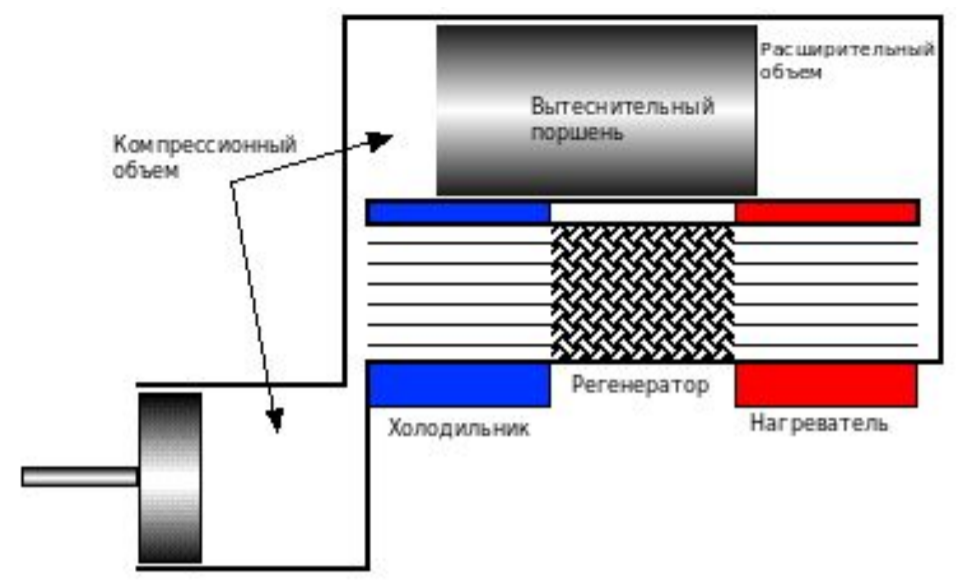
\includegraphics[width=.65\linewidth]{Lab4_2.png}
				\caption{Схема работы двигателя Стирлинга $\gamma$ типа}
				\label{fig1}
			\end{figure}
		
			Идеальный двигатель Стирлинга работает по циклу Стирлинга, который вместе с циклом Карно приведен ниже.
			\begin{figure}[h!]
				\centering
				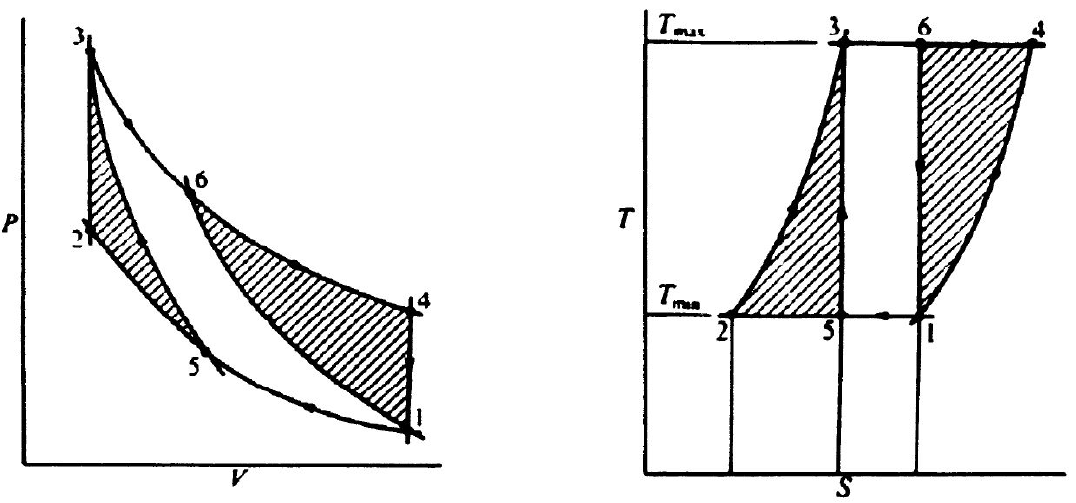
\includegraphics[width=.75\linewidth]{Lab4_1.png}
				\caption{Схема подключения проволоки}
				\label{fig2}
			\end{figure}
		
			Где процессы:
			\begin{itemize}
				\item 1-2 -- изотермическое сжатие с отдачей тепла с отдачей тепла во внешнюю среду
				\item 2-3 -- изохорный нагрев за счет тепла в регенераторе
				\item 3-4 -- изотермическое сжатие с получением тепла от нагревателя
				\item 4-1 -- изохорное охлаждение с передачей тепла регенератору
			\end{itemize}
		
			КПД можно определить по формуле:
			\begin{equation}
				\eta = \frac{A}{Q}
			\end{equation}
			где $A$ - работа, совершаемая телом за цикл, $Q$ - подведенное тепло.
			
			Работу можно найти как площадь, ограниченную циклом в p-V координатах:
			\begin{equation}
				A = \nu R T_\text{н} \ln(\frac{V_2}{V_1}) - \nu R T_x \ln(\frac{V_2}{V_1})
			\end{equation}
			Тепло подводится на участке 3-4, поэтому:
			\begin{equation}
				Q = Q_{34} = \nu R T_\text{н} \ln(\frac{V_2}{V_1})
			\end{equation}
			
			Отсюда кпд цикла:
			\begin{equation}
				\nu = 1 - \frac{T_x}{T_\text{н}}
			\end{equation}
	\section{Измерение согласованного сопротивления}
		\subsection{Ход работы}
			Для измерения согласованного сопротивления двигатель стирлинга оборудовался нагрузкой с переменным сопротивлением, на которой с помощью осциллографа измерялось напряжение. Было проведено несколько экспериментов с различными значениями сопротивления, для того, чтобы потом можно было определить наибольшую мощность
		\subsection{Обработка данных}
			По полученным данным, был построен график зависимости мощности двигателя от сопротивления реостата.
			\begin{figure}[h!]
				\centering
				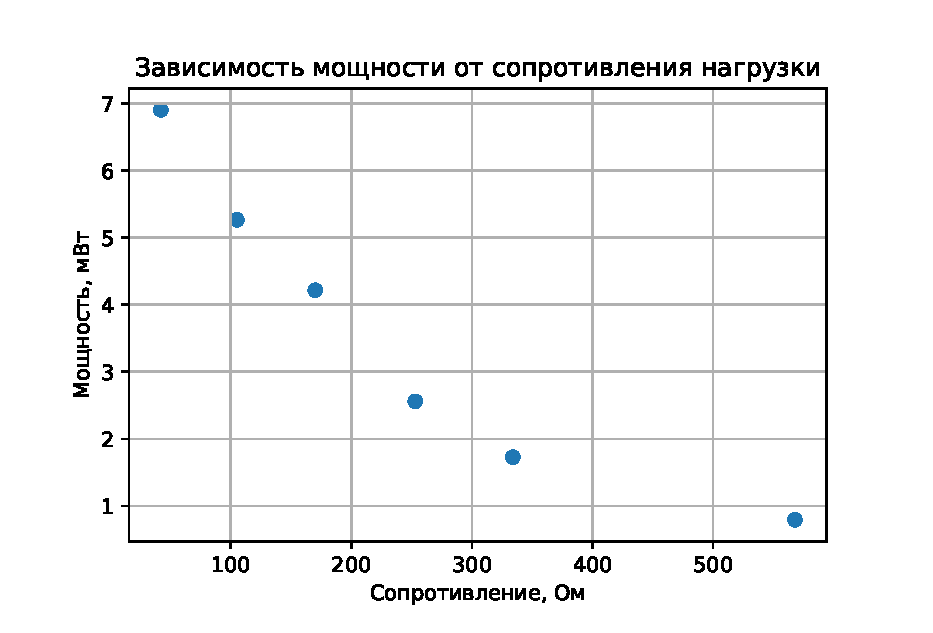
\includegraphics[width=.85\linewidth]{Lab4_2.eps}
				\caption{}
				\label{fig4}
			\end{figure}
		
			Максимальная мощность наблюдается при сопротивлении нагрузки $R \approx 42 \text{Ом}$(конечно, стоило продожить измерение нагрузки при меньших сопротивлениях, но имеем что имеем), откуда получаем, что экспериментальный КПД:
			\begin{equation}
				\eta = \frac{P_{max} \Delta t}{q \Delta m} \approx 0.7 \%
			\end{equation}
	\section{Построение p-V диаграмы}
		\subsection{Ход работы}
			В ходе работы, к установке с оптимальным сопротивлением были подключены оптодатчик и датчик давления, которые позволили фиксировать положительные отклонения от атмосферного давления, а так же с хорошей точностью определить период цикла. 
		\subsection{Обработка данных}
			Для построения $p-V$ диаграммы мы использовали параметрические зависимости $p(T), V(T)$. С $p(T)$ все просто: к камере двигателя подключался датчик давления, который фиксировал положительные отклонения от атмосферного давления. График таких давлений представлял из себя синусоиду с отсутствующей отрицательной частью, я его дополнил, отразив относительно нуля и сместив на четверть периода. Далее я предположил, что зависимость $V(T)$ это та же синусоида, только со смещенной фазой и, естественно, другой амплитудой. Амплитуда была найдена исходя из разности объемов закрытого и открытого поршня. Таким образом, мы получили зависимости $p(T), V(T)$. Построим с их помощью график $P(T)$:
			\begin{figure}[h!]
				\centering
				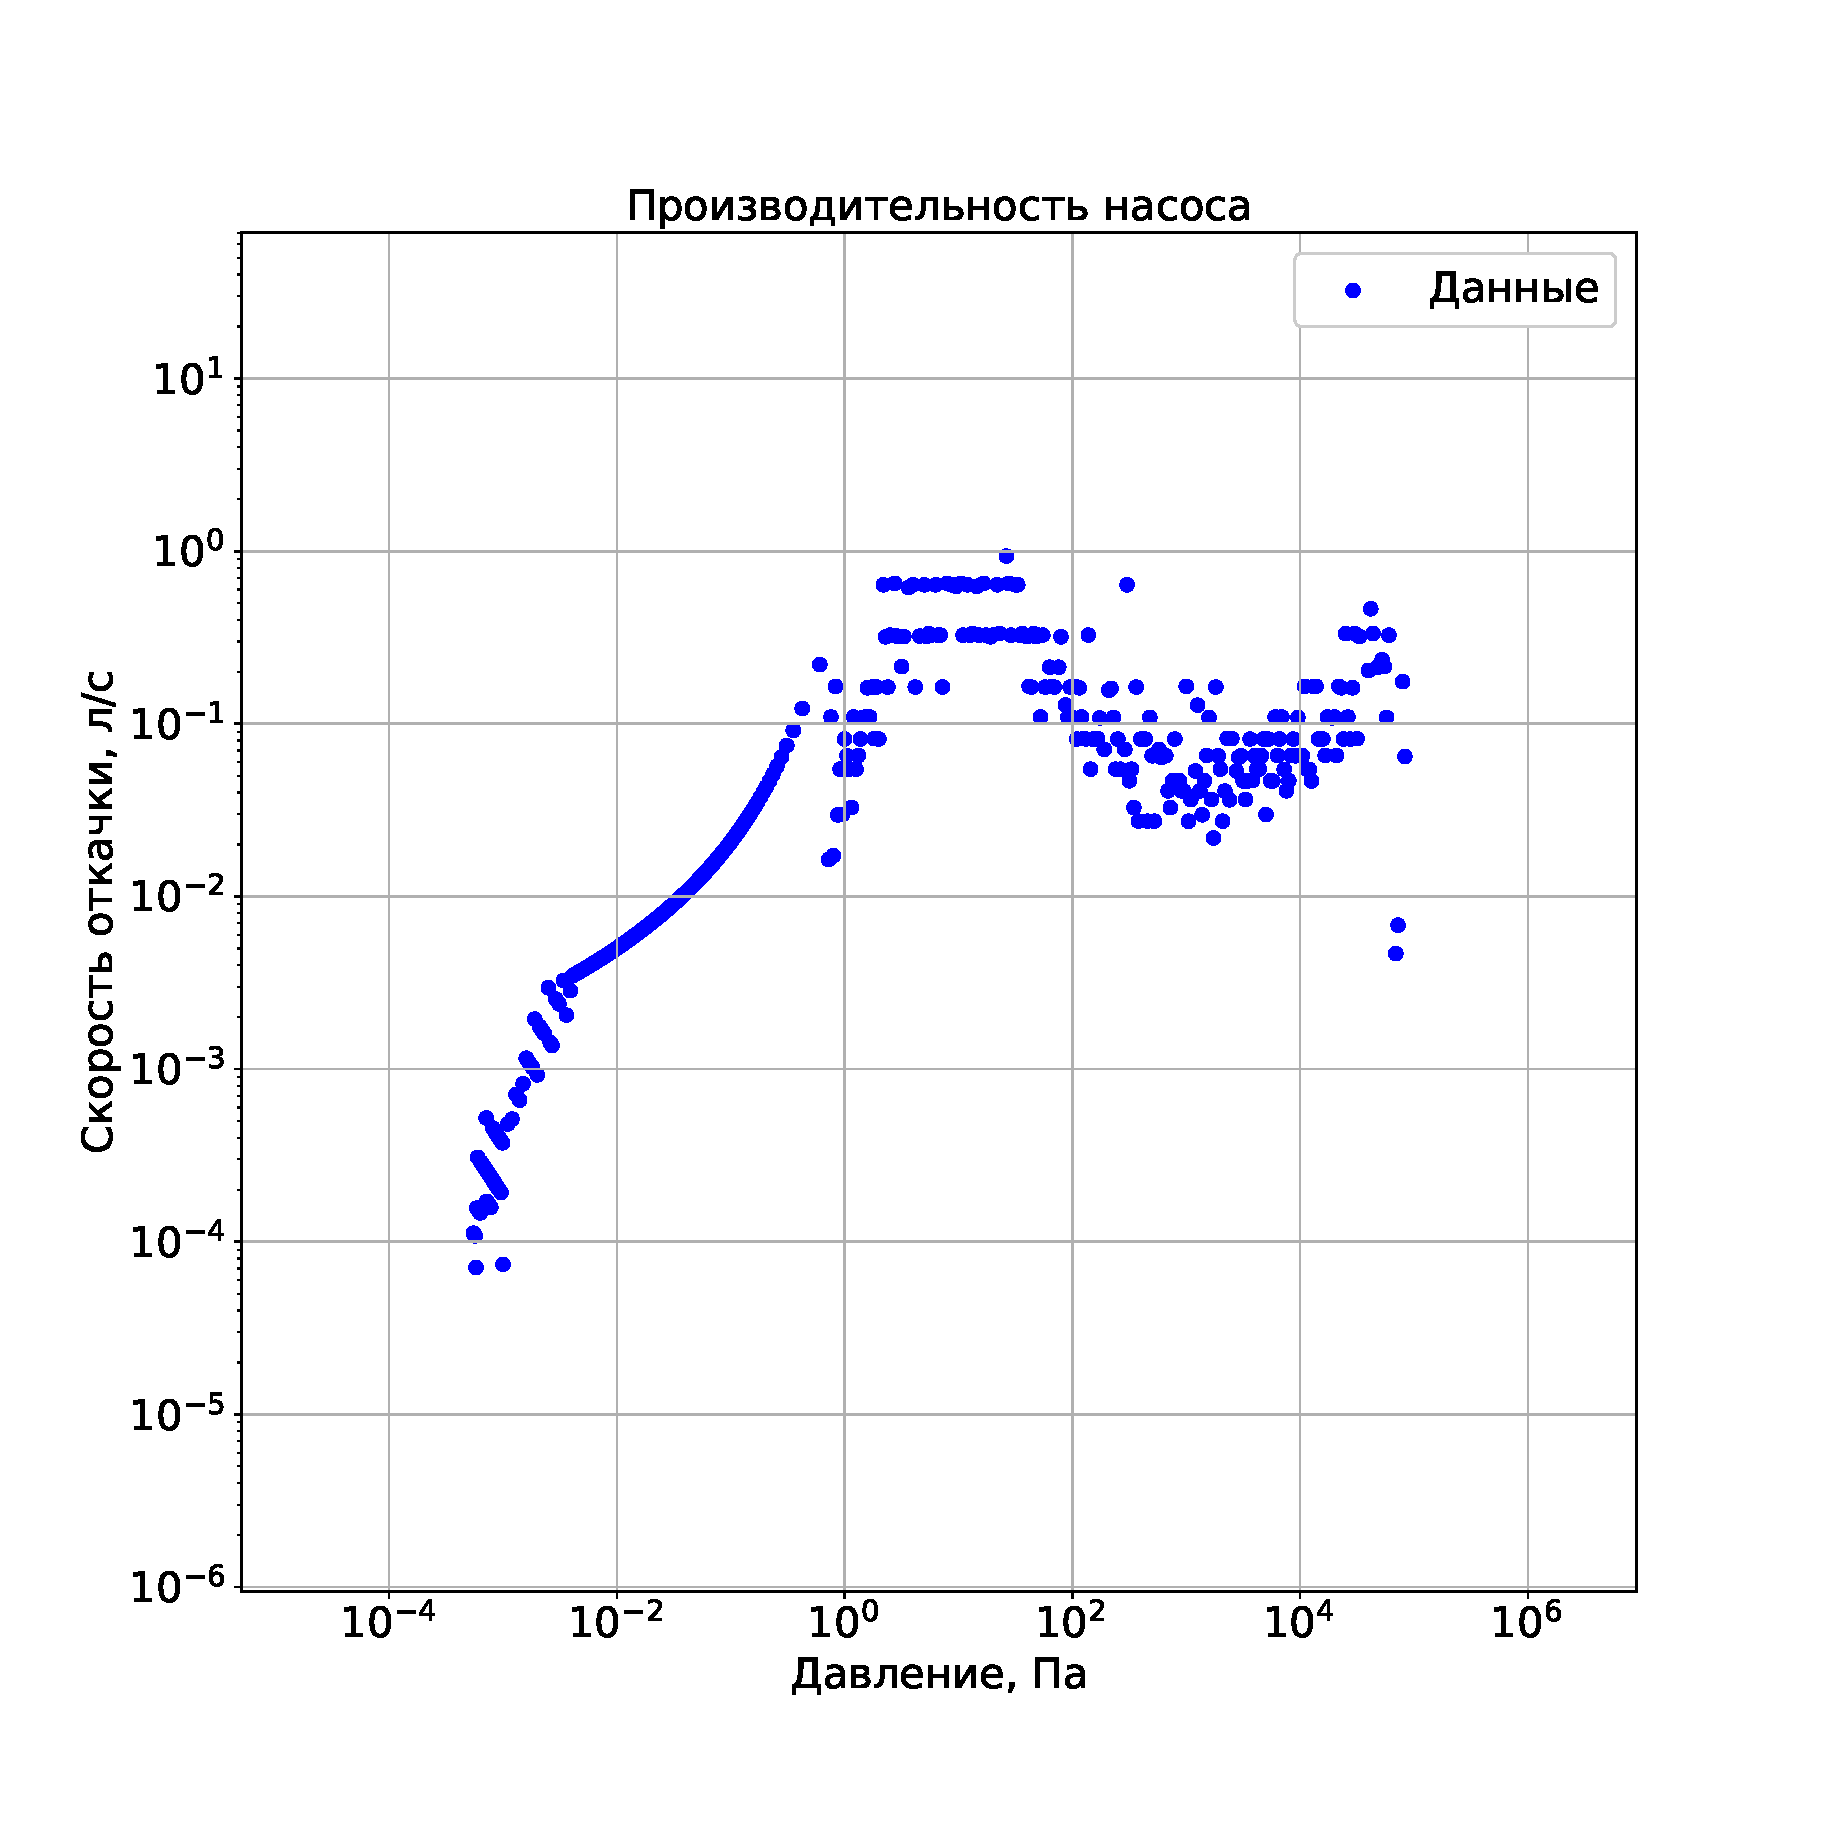
\includegraphics[width=.85\linewidth]{Lab4_1.eps}
				\caption{$p-V$ диаграмма}
				\label{fig6}
			\end{figure}
		
			Ожидаемо, получился эллипс. Посчитаем КПД такого цикла:
			\begin{equation}
				\eta = \frac{S_A}{S_Q} \approx 3.44 \%
			\end{equation}
			Где $S_A$ - площадь эллипса (работа газа в цикле), а $S_Q$ - сумма площади под эллипсом и площади эллипса (теплота, подводимая к газу в цикле)
	\section{Выводы}
		\begin{itemize}
			\item Фактический КПД, получившийся экспериментальным путем отличается от КПД цикла, построенного в предположении, что $V$ меняется со временем по синусоиде примерно в 5 раз. Это отличие может означать, что имеют место различного рода потери, кроме того, возможно было выбрано неверное сопротивление нагрузки. Тем не менее, полученные результаты отличаются не более чем на порядок, поэтому указанная модель может быть применима для грубой оценки КПД такого двигателя. 
			\item Теоретический КПД, как и теоретический $p-V$ цикл сильно расходятся с экспериментальными. Формулы из теории выведены в предположении идеальной тепловой машины, работающей по циклу Стирлинга, в нашем случае, теория неприменима из-за большого количества неидеальных элементов нашей машины, например, спирт, который сжигается в спиртовке нагревает в том числе окружающую среду, что, разумеется сильно влияет на КПД двигателя. 
		\end{itemize}
\end{document}